%!TEX root = ../../../main.tex

\section{Photoluminescence spectra} \label{sec::spectra}

	To identify \nds containing \sivs, we performed confocal scans of the samples.
	To reduce bias in the measurements, not only the brightest spots of the confocal scans are investigated, but also those which barely exceed \bkg fluorescence.
	\sivs are further investigated by measuring \pl (PL) spectra, single photon statistics and photostability.
	As discussed in \autoref{ch::sivs}, the typical luminescence spectrum of an \siv is composed of a prominent \zpl peak and weak sidebands.
	Investigations of both are reported independently in the following paragraphs.

\subsection{\Zpl}\label{subsec::zpl}

	The \cwl and the \lw of the \zpl (\ZPL) of SiV luminescence spectra for samples \insituF, \insituS, and \insituH are determined by fitting a Lorentzian fit to the \ZPL.
	Both spectra from single and multiple \sivs are taken into account.
	In \autoref{fig::bimodal_distr} the \lw for each measured \ZPL is plotted against its \cwl.

	\begin{figure}[htp]
			\centering
			\testbox{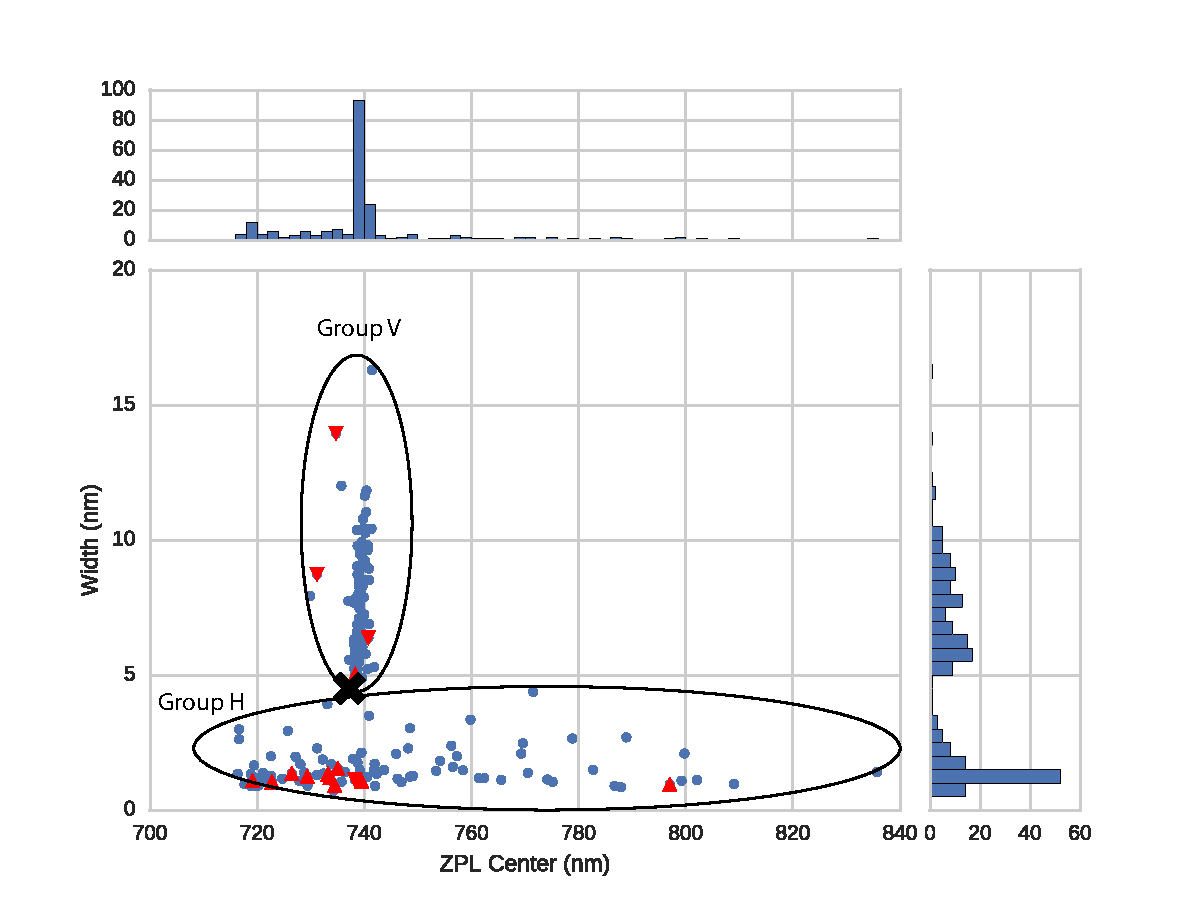
\includegraphics[trim = 0 0 0 0,  clip= true, width = 0.7\linewidth]{./pics/distro_histo_sarah.pdf}}
			\caption[Spectral distribution of \siv \ZPLs]{Distribution of the \ZPL \cwl versus the \lw of the \ZPL of the investigated \sivs in milled \nds containing \textit{in-situ} incorporated \sivs for samples \insituF, \insituS, \insituH{}. The data seperates into a horizontal (\hl) and a vertical (\vl) cluster. The bold black cross marks the position of an ideal \siv in unstrained bulk diamond \cite{Arend2016a}. The red triangles indicate emitters with an antibunching dip in the \gtz measurement. Upwards pointing triangles represent blinking emitters (fluorescence intermittency), while triangles pointing down represent non-blinking emitters (see \autoref{subsec::photostab}).}
			\label{fig::bimodal_distr}
	\end{figure}

	What immediately strikes the eye is a pattern that to our knowledge has not been reported to date:
	The observed \ZPLs partition into two groups, dentote a horizontal lobe (\hl) and a vertical lobe (\vl). The two lobes are seperated by a gap, i.e.\ a region with a pronouced lack of data points.
	Single emitters are identified both in \hl and \vl, marked as red triangles in \autoref{fig::bimodal_distr}. Further details on single emmiters are given in section \autoref{subsec::g2}.
	\\
	The two groups are defined by their characteristic \cwls and \lws:
	In \hl very prominent \ZPL peaks are found showing \lws in the range of \SIrange{1}{5}{nm} and \cwls in the range of \SIrange{715}{835}{nm}.
	\autoref{subfig::emnarrow} shows a representative spectrum of a single emitter in \hl (denoted \emnarrow), exhibiting a \ZPL line width of \SI{1.4}{nm} and a \cwl of \SI{726.5}{nm}.
	In contrast, in \vl, the spectra exhibit broader \ZPL \lws of approximately \SI{5}{nm} up to \SI{18}{nm}.
	Their \ZPL \cwls, however, are distributed within the very narrow range of \SIrange{738}{741}{nm}.
	\autoref{subfig::embroad} shows a spectrum of a single emitter of \vl (denoted \embroad) with a ZPL \lw of \SI{6.4}{nm} and a \cwl of \SI{740.8}{nm}.
	For comparison, the room temperature ZPL of \sivs in unstrained bulk diamond exhibits a \lw of \SIrange{4}{5}{nm} and a \cwl of \SI{737.2}{nm} marked with a black cross in \autoref{fig::bimodal_distr} \cite{Arend2016a,Dietrich2014}.

	\begin{figure}[htp]
		\begin{subfigure}[tp]{0.45\linewidth}
			\centering
			\testbox{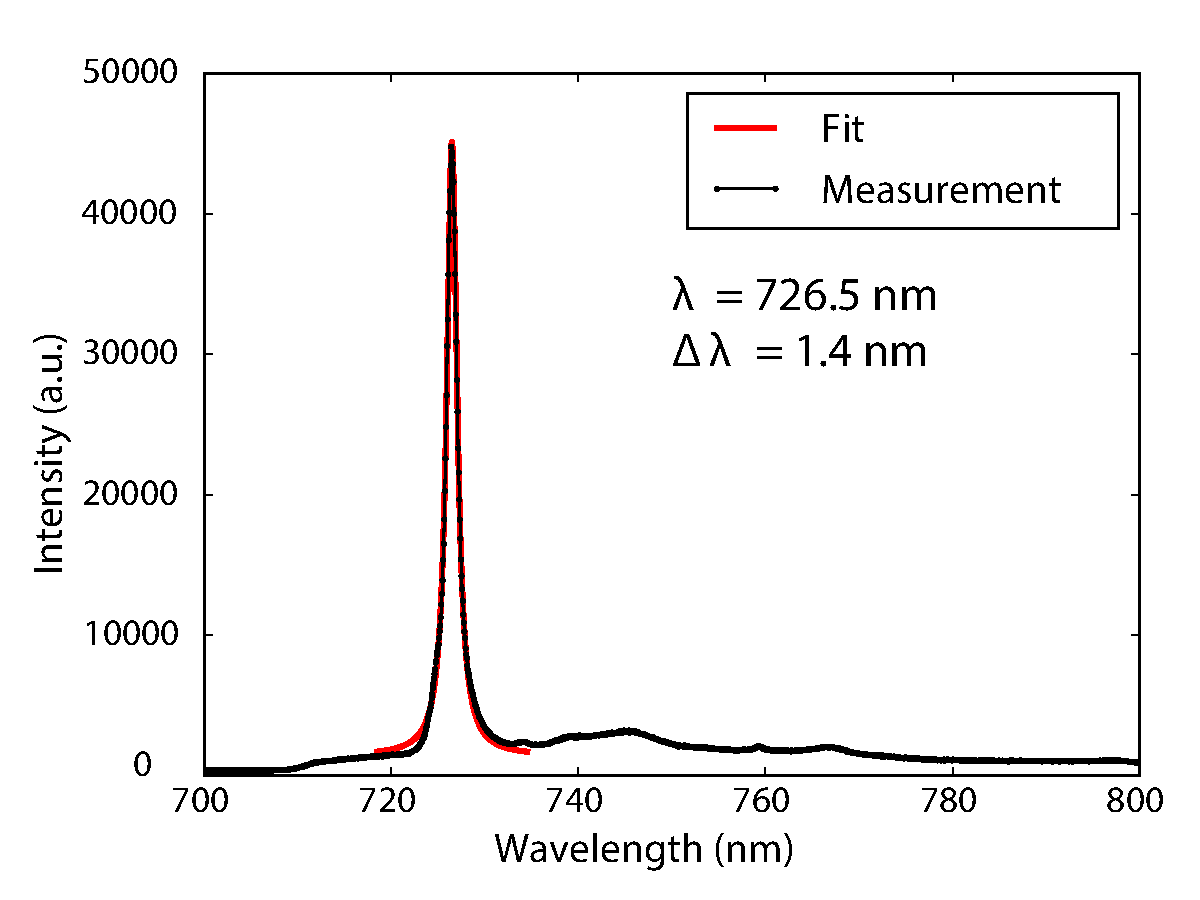
\includegraphics[trim = 0 0 0 0 , clip = true, width = \linewidth]{./pics/Ir8_Spektrum_8_notitle.pdf}}
			\caption{}\label{subfig::emnarrow}
		\end{subfigure}
		\hfill
		\begin{subfigure}[tp]{0.45\linewidth}
			\centering
			\testbox{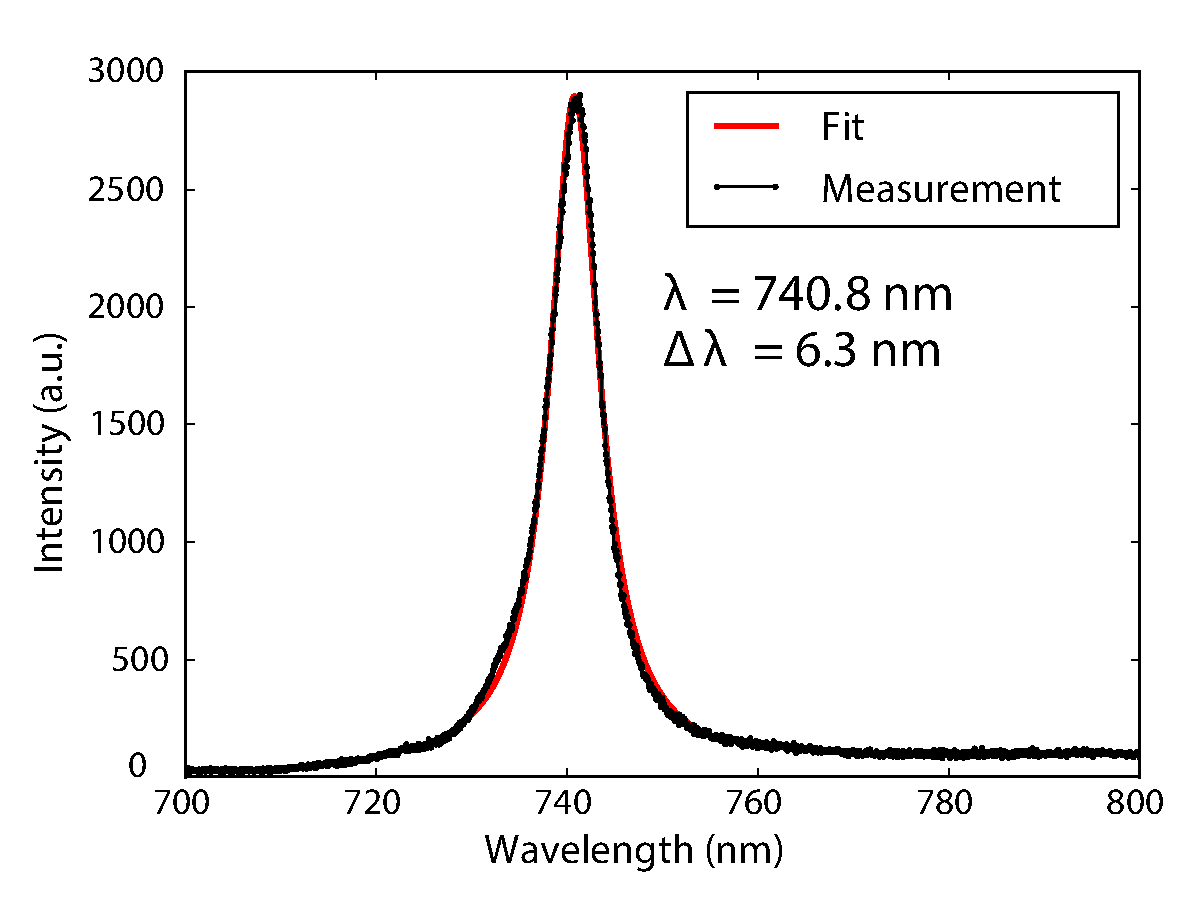
\includegraphics[trim = 0 0 0 0,  clip = true, width = \linewidth]{./pics/Ir8_scan_xy05_199uW_t30_notitle.pdf}}
			\caption{}\label{subfig::embroad}
		\end{subfigure}
		\caption[Sample \siv \pl spectra for \vl and \hl]{Representative photoluminescence spectra of sample \insituHao measured at room temperature. (a) Spectrum of \hl of \autoref{fig::bimodal_distr}, denoted \emnarrow. (b) Spectrum of \vl of \autoref{fig::bimodal_distr}, dentoted \embroad. The red lines are Lorentzian fits to the peaks.}
		\label{fig::spectra}
	\end{figure}

	To determine how much the \ZPLs contribute to the total observed emmision of \emnarrow and \embroad, we determine the \db factors for both.
	The \db factor is defined by $DW = I_{ZPL}/I_{TOT}$ and is therefore suited as a measure for sideband intensity.
	The \db factor for \emnarrow amounts to \num[separate-uncertainty]{0.81(1)} (given uncertainty due to fit).
	This \db factor corresponds to a \hr factor $S =- \ln{(DW)}$ \cite{Walker1979} of \num[separate-uncertainty]{0.21(1)}, which is in good agreement with the values reported in \cite{Neu2011b}.
	The error is mainly due to background corrections.
	When zooming in onto the spectrum of \embroad we do not find distinct sidebands peaks, i.e.\ almost all emission for this emmiter is alloted to the \ZPL.
	Considering resolution limits of the spectrometer, darkcounts and fluorescence background, we evaluate the \db factor to be larger than \num[separate-uncertainty]{0.97}.
	It is the largest \db factor amongst all our milled \sivs.
	The two mentioned \db factors should not be interpreted as single representative emitters for the respective groups, they rather serve as an orientation of the spread of the \db factors of both groups.
	It has to be pointed out, that we did not find any systematic difference of the \db factor between \hl and \vl.
	\\
	To provide context for the novel findings presented in \autoref{fig::bimodal_distr}, we compare our results to various earlier findings.
	Furthermore, we discuss an additional comparison to an investigated control sample fabricated using \si implantation.
	The resuls are presented in \autoref{fig::bimodal_distr_compare}.


	\begin{figure}[htp]
		\centering
		\testbox{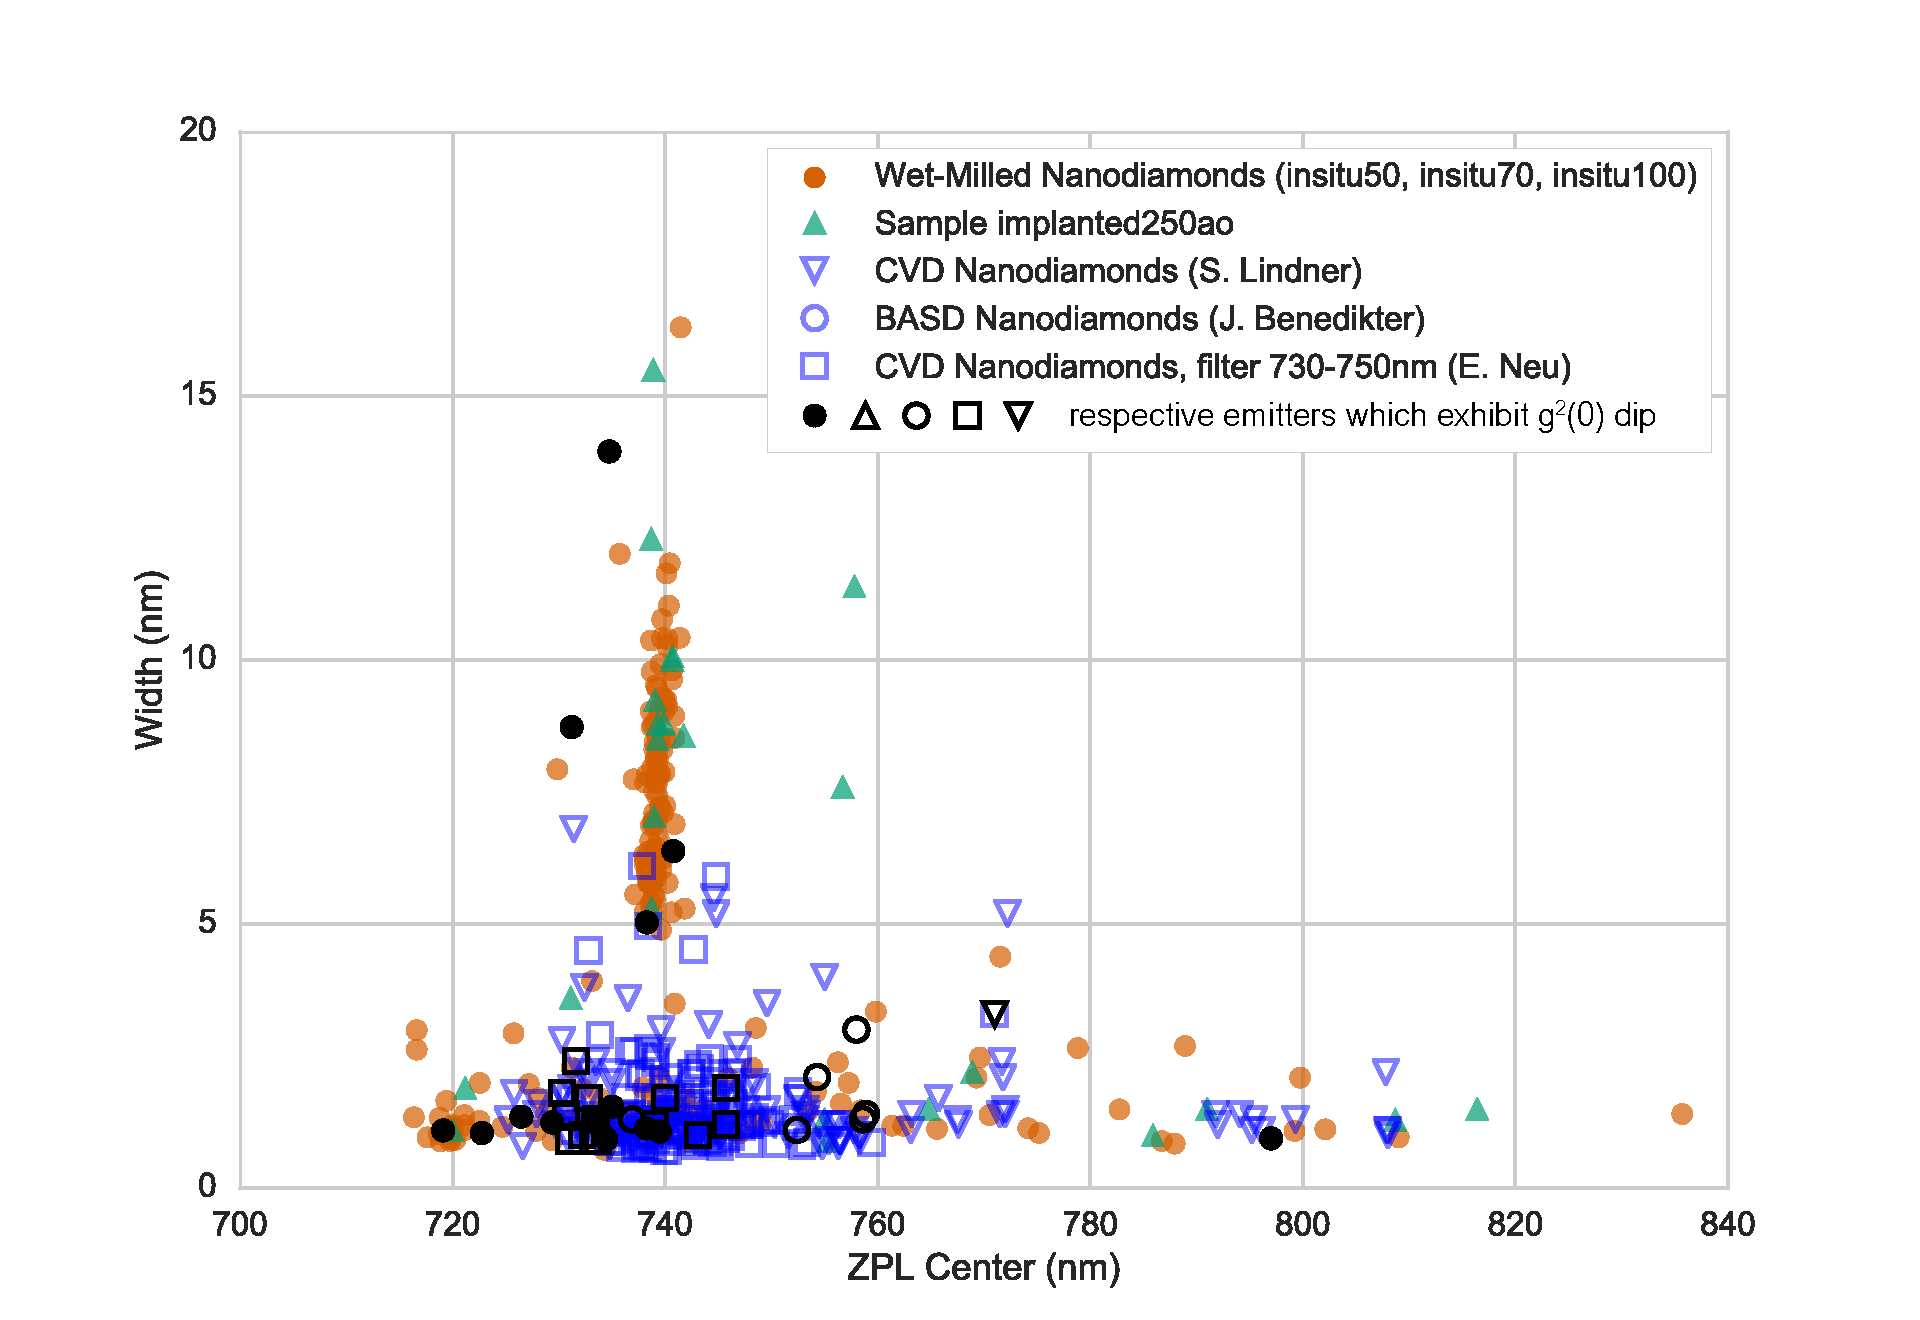
\includegraphics[trim = 0 0 0 0,  clip= true, width = 0.7\textwidth]{./pics/distro_alldata_three_colors_legend.pdf}}
		\caption[Comparison of obtained \siv \lws with available data sources]{Comparison of the distribution of the \lw vs. the center wavelength of the ZPL of the investigated \sivs in milled \nds (samples \insituF, \insituS, \insituH) with data measured on sample \implantedTao (implanted with \Si); with data measured in our group on CVD \nds produced by M. Schreck \cite{Neu2011b}; with data measured on \nds reported by J. Benedikter in \cite{Benedikter2017a}; and with data measured in CVD diamonds by E. Neu in a filter window between \SIlist{730; 750}{nm} \cite{Neu2012}. Black symbols represent emitters exhibiting a dip in the \gtz function, indicating a single or very few \sivs}
		\label{fig::bimodal_distr_compare}
	\end{figure}


	Samples for which previous data has been taken are:
	\begin{enumerate}
		\item \nds produced by \basd (BASD) of polycrystalline \CVD diamond films (blue rings in \autoref{fig::bimodal_distr_compare} \cite{Neu2011a}; data taken from \cite{Benedikter2017a})
		\item \label{item::elke_cvd}\nds produced directly via a \CVD process with \textit{in-situ} incorporated \sivs; measured in a spectral filter window of \SIrange{730}{750}{nm} (blue squares in \autoref{fig::bimodal_distr_compare}; data reused from \cite{Neu2012} with permission)
		\item \nds produced in the same manner as the \CVD sample in \ref{item::elke_cvd} (blue downwards pointing triangles in \autoref{fig::bimodal_distr_compare}; produced by M. Schreck \cite{Neu2011b}; spectroscopic measurement performed with setup described in \autoref{sec::methods})
	\end{enumerate}
	All previous data from different \nd material fit nicely with the \ZPL distribution presented in \autoref{fig::bimodal_distr_compare}, confirming the findings of \autoref{fig::bimodal_distr}.
	\\
	We verify that the observed luminescent defects are indeed \si related by performing control experiments with \si implanted samples (sample \implantedTao).
	By doing so we rule out the possibility that the two lobes in the distribution are a result of artifacts.
	Such artifacts include other elements incorporated into the \nds during the growth process: Residue from previous processes performed in the diamond growth chamber or material from chamber parts may be incorporated during \nd growth.
	\autoref{fig::bimodal_distr_compare} shows that the implanted \sivs cover roughly the same spectral range as the \textit{in-situ} incorporated centers from around \SIrange{720}{820}{nm} as the \textit{in-situ} incorporated centers.
	This correlation provides strong evidence for the \si related origin of the defects.
	\\
	% In the next paragraphs, the \ZPL distribution will be discussed in further detail.
	To provide a theoretical interpretation, the \ZPL \cwl shift is investigated in further detail and compared to results from density functional calculations.
	Zooming in to \vl (\autoref{subfig::distro_inset1}) it becomes clear that only six of the measured data points in \vl are situated at a shorter \cwl than the point attributed to an ideal \siv in unstrained bulk material.
	The the shortest wavelength shift is at \SI{729.9}{nm}.
	At the same time, much more data exhibit a \cwl bigger than the ideal \siv.
	This asymmetry suggests that a red-shift of the \ZPL of an \siv is significantly more likely than a blueshift.

		\begin{figure}[htp]
			\begin{subfigure}{.5\textwidth}
				\centering
				\testbox{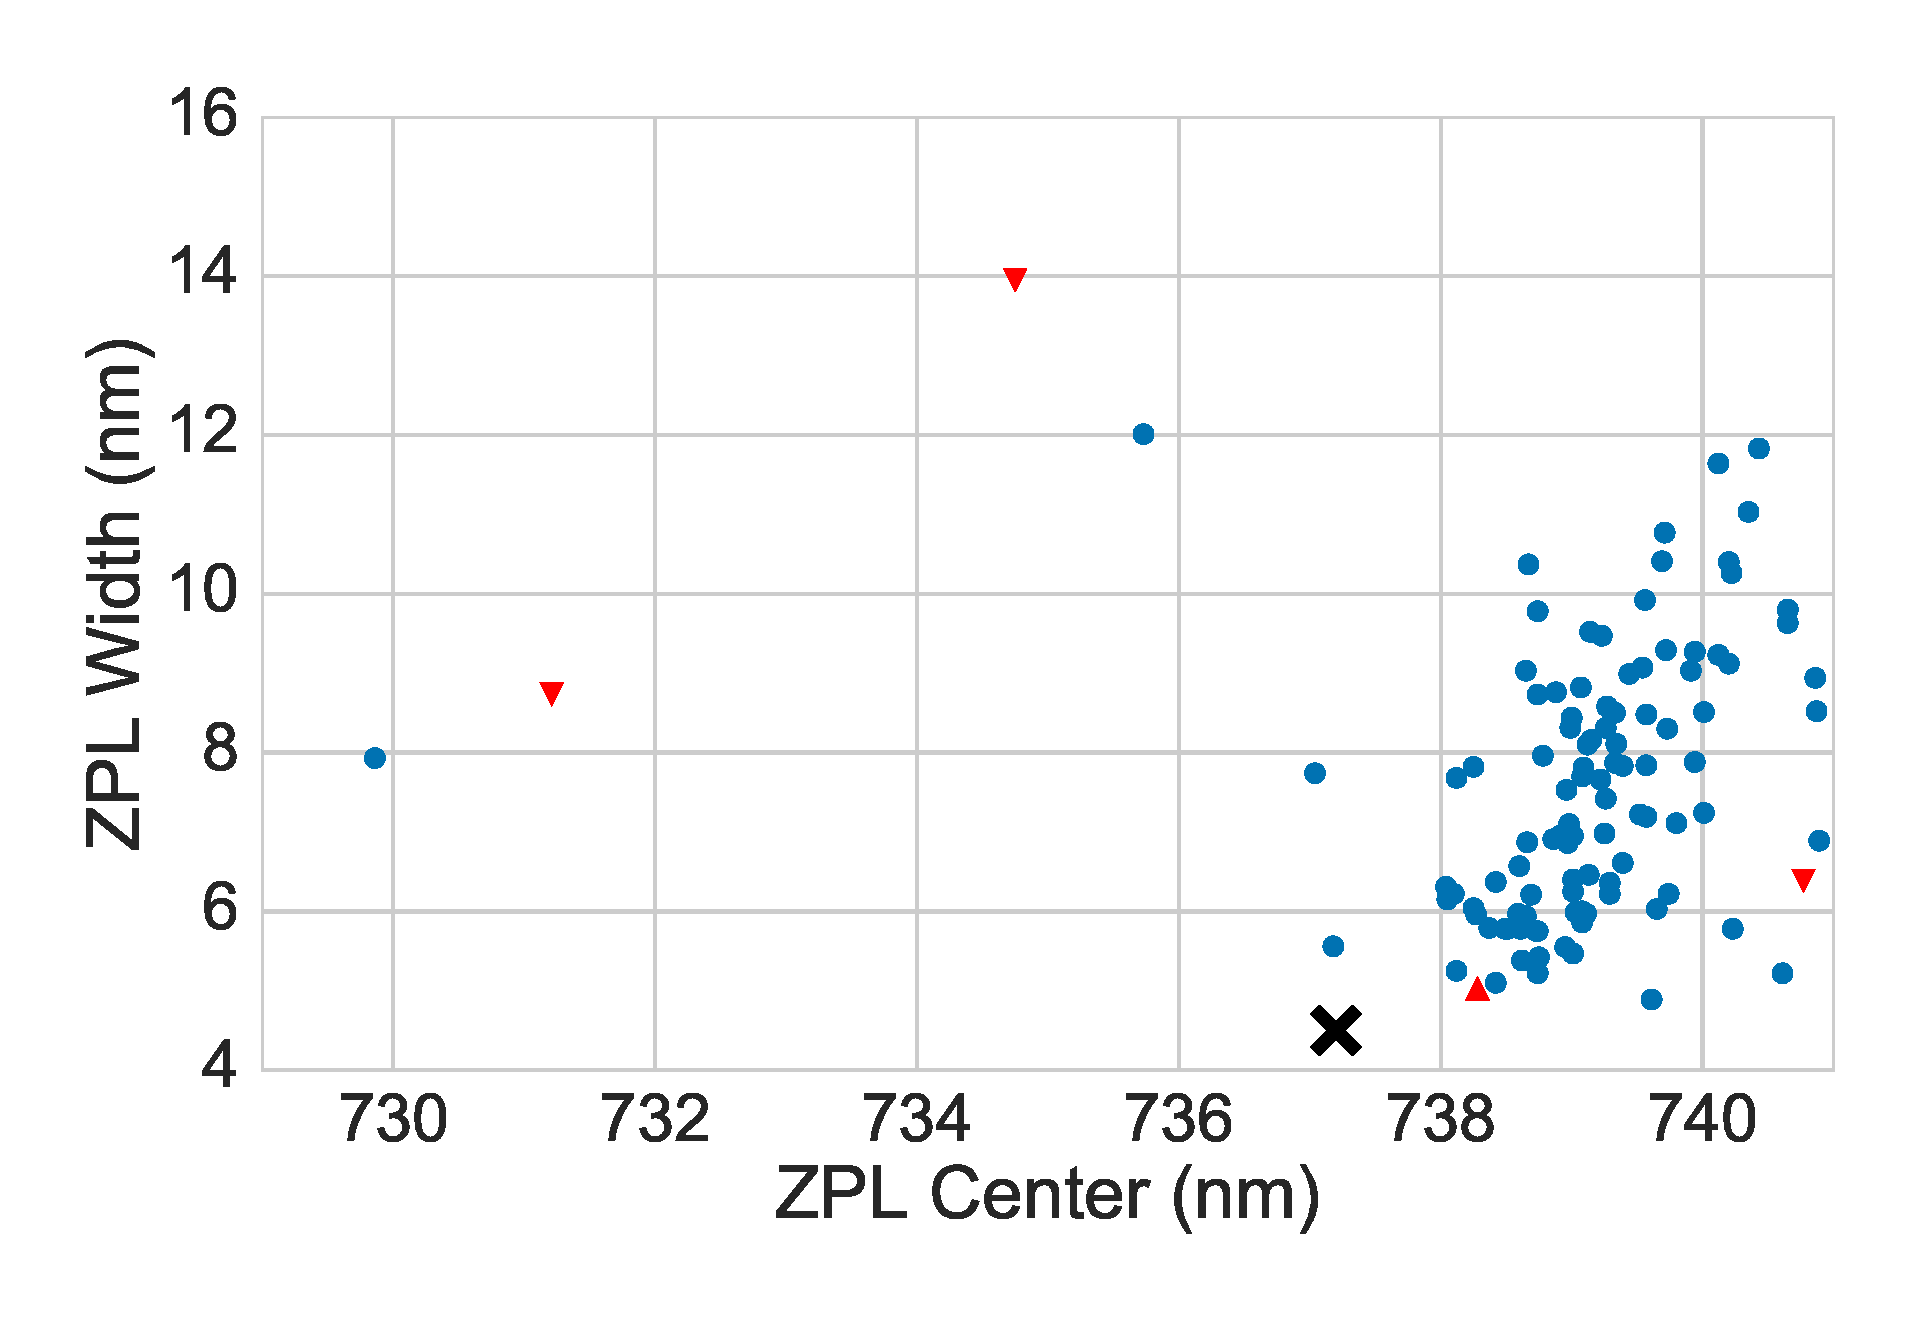
\includegraphics[trim = 0 0 0 0,  clip= true, width=0.9\linewidth]{./pics/paper_inset_line_statistics_nofit.pdf}}
				\caption{}
				\label{subfig::distro_inset1}
			\end{subfigure}
			\begin{subfigure}{.5\textwidth}
				\centering
				\testbox{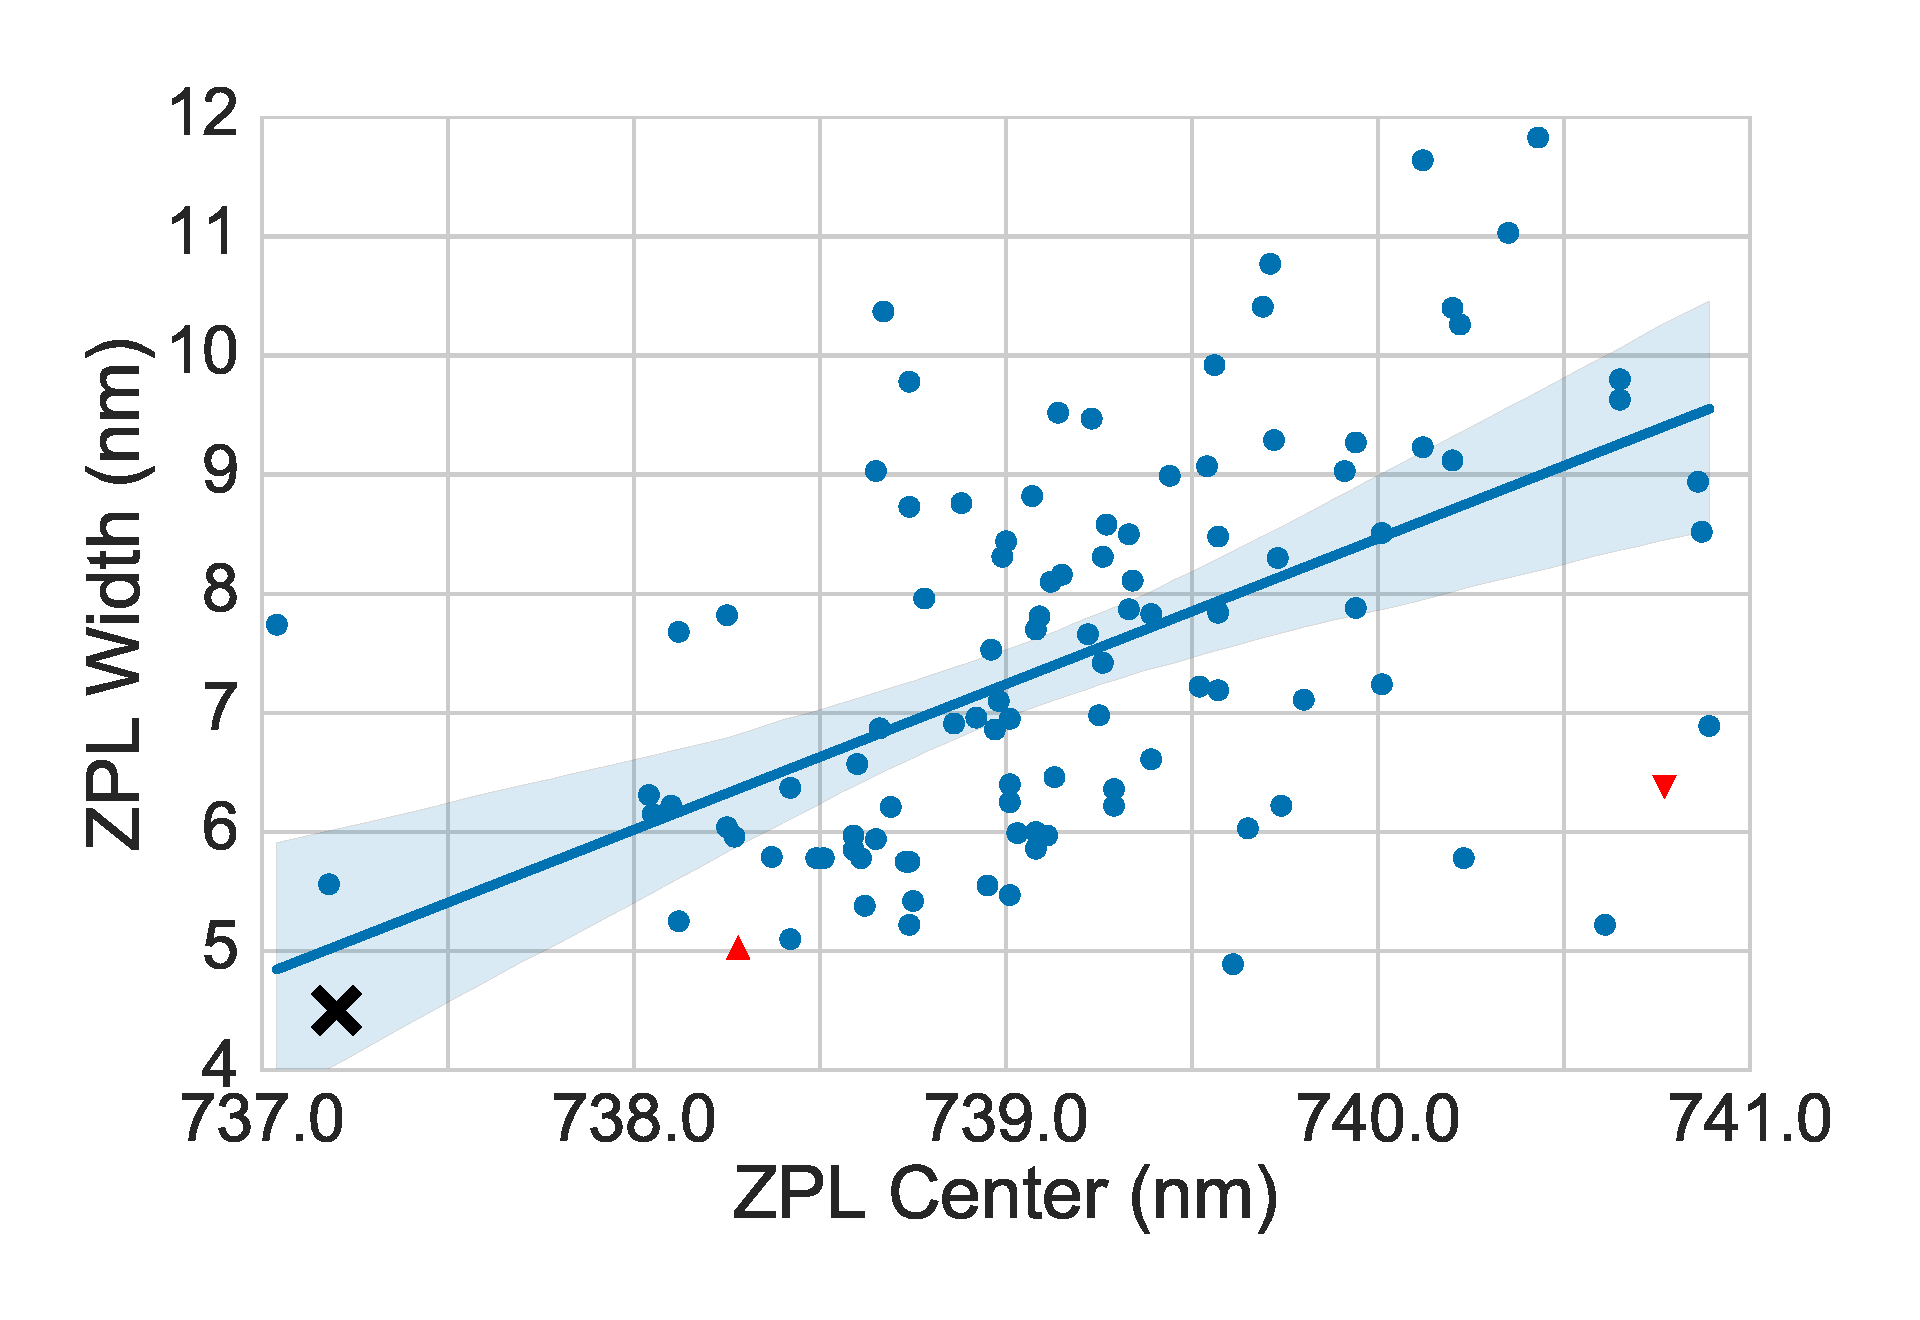
\includegraphics[trim = 0 0 0 0,  clip= true, width=0.9\linewidth]{./pics/paper_line_statistics_regression.pdf}}
				\caption{}
				\label{subfig::distro_inset2}
			\end{subfigure}
			\caption[Zoom-in onto \sivs of the \vl]{(a) A zoom into \vl. While many data points exhigit higher \cwls (i.e. a redshift) than the ideal \siv in bulk, only few exhibit shorter \cwls (i.e. a blueshift). (b) Zooming further into \vl, a clear trend of broader \ZPL \lws for larger \ZPL center shifts is visible. The line in a linear regression to all datapoints between \SIlist{737;741}{\nano\meter} which exhibit a \lw bigger than \SI{4}{\nano\meter}.}
			\label{fig::bimodal_distr_zoom}
		\end{figure}

	Several mechanisms contribute to the \cwl shift, predominantely hydrostatic- and material strain.
	As explained in \autoref{subsec::raman}, we measured the Raman shift of samples \insituS and \implantedTao.
	These measurements indicate strain in the diamond lattice in the range of \SIrange{-8.56}{4.26}{\giga\pascal}.
	\autoref{fig::stress_pressure} shows results from density funtional calculations.
	The shift of the  \ZPL is modelled in dependence of pressure in the diamond lattice both for hydrostatic stress and for uniaxial stress.
	\autoref{fig::stress_pressure} illustrates that the assumption stated in \autoref{subsec::raman}, namely that the strain in the \nds is due to hydrostatic and uniaxial stress, corresponds well with the measured \ZPL shifts in \vl.

		\begin{figure}[htp]
			\centering
			\testbox{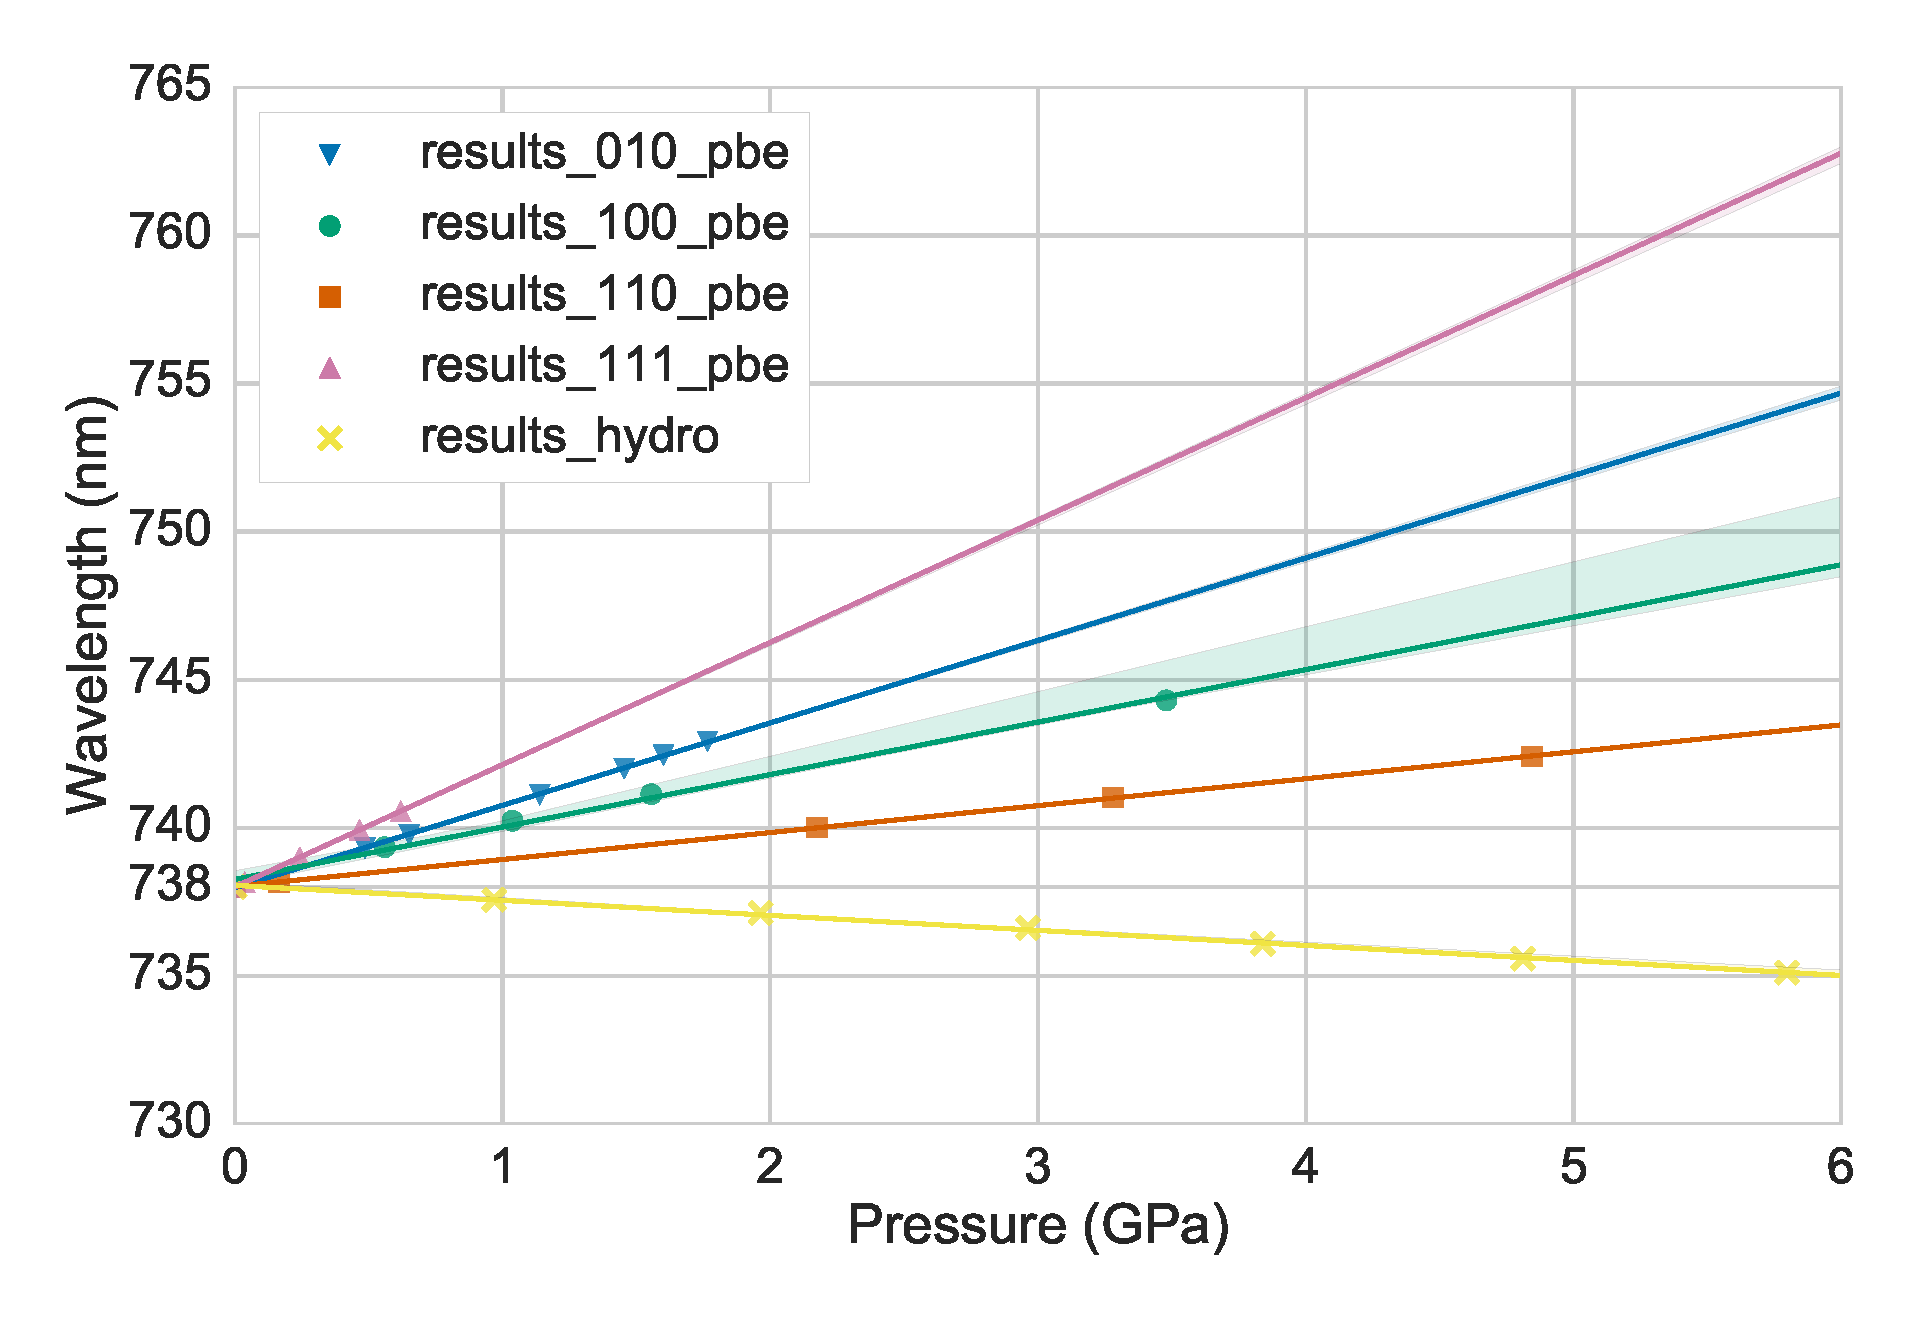
\includegraphics[trim = 0 0 0 0,  clip= true, width = 0.5\textwidth]{./pics/adam_gali_big_labels.pdf}}
			\caption[Calculated dependence between \siv \ZPL and lattice pressure]{Calculations of the wavelength of the \siv \ZPL in dependence of pressure. Markers: calculated pressure with PBE functional; Lines: linear fits to the calculated points, the shaded area around the lines representing the one sigma (68\%) confidence intervall. Yellow: hydrostatic pressure; other colors: uniaxial pressure, for different orientations. All calculations are performed with a PBE functional. Hydrostatic-type pressure causes a moderate blue shift whereas uniaxial strain causes larger redshift with different magnitudes depending on the direction of the strain}
			\label{fig::stress_pressure}
		\end{figure}

	With higher uniaxial pressure, the \ZPL becomes more and more red-shifted.
	The blueshifted \ZPL \cwls are explained by hydrostatic stress in the diamond material.
	The strain calculated from the Raman measurements corresponds well with the results in \autoref{fig::stress_pressure} for \vl.
	However, the measured shifts in \hl are too broad to be solely explained by strain in the diamond.
	A potential explanation for the very broad distribution of defect center \ZPL \cwls could be the association of \sivs with a further nearby defect, such as a vacancy, or a modified SiV complex such as SiV:H \cite{Thiering2015}.
	\\
	Zooming in to \vl, another effect becomes visible (\autoref{subfig::distro_inset2}):
	With increasing  \ZPL \cwl, the \lw becomes broader.
	As discussed above, a red-shift of the \ZPL is linked to increasing uniaxial strain.
	Thus we conclude that the \ZPL \lw too is affected by strain in the diamond lattice.
	Here, a modified electron-phonon coupling \cite{Jahnke2015a} causes increased uniaxial stress, resulting in larger \lws.
	A similar effect has been previously observed for \sivs at cryogenic temperatures \cite{Arend2016a}.
	\\
	To conclude, we are able to explain the distribution of \ZPL \cwls in \vl very consistently with theoretical predictions based on perturbative shifts due to strain in the diamond lattice.
	On the other hand, we have to assume that \hl is comprised of modified \sivs, the structure of which is currently unclear.
